\documentclass{article}
\usepackage[utf8]{inputenc}
\usepackage[spanish]{babel}
\usepackage{listings}
\usepackage{graphicx}
\graphicspath{ {images/} }
\usepackage{cite}

\begin{document}

\begin{titlepage}
    \begin{center}
        \vspace*{1cm}
            
        \Huge
        \textbf{Proyecto Parcial 1}
        
        \textbf{Manual de instrucciones}
            
        \vspace{0.5cm}
        \LARGE
        Informática II
            
        \vspace{1.5cm}
            
        \textbf{Reinaldo Marín Nieto}


        \textbf{Jonathan Macías Díaz}
            
        \vfill
            
        \vspace{0.8cm}
            
        \Large
        Despartamento de Ingeniería Electrónica y Telecomunicaciones\\
        Universidad de Antioquia\\
        Marzo de 2021
            
    \end{center}
\end{titlepage}

\tableofcontents
\newpage
\section{Componentes del proyecto}\label{intro}
Para el correcto funcionamiento del proyecto, se usan los siguientes componentes:


-Placa Arduino UNO


-Protoboard


-2 Circuitos Integrados 74HC595


-64 LEDs


-8 resistencias de 560 ohms

\section{Menú Principal} 
Cuando ejecutemos la simulación, automáticamente se nos abrirá un menú con distintas opciones, escribiendo su número correspondiente nos dirigiremos hacia esa función.

Bienvenido al menú principal, selecciona una opción:

1.Verificación
2.Ingresar patrón.



\section{Funciones} \label{contenido}
Luego de seleccionar una opción, nos dirigiremos a una función del proyecto. Una función es una serie de instrucciones preconstruidas que fueron programadas para que el proyecto las ejecute y genere el resultado esperado.


\subsection{Verificación}
Esta función no requiere datos adicionales, se trata de una serie de instrucciones que se compilan para encender todos los LEDs de la matriz 8x8 al mismo tiempo. Su propósito principal es la de asegurarse que todos los LEDs y los componentes implicados funcionan correctamente
\subsection{Ingresar Patrón}
Esta función permite al usuario ingresar una serie de datos binarios para representar un patrón completamente personalizado.

Para ejecutarse correctamente, el usuario debe ingresar unos (1) para los LEDs que quiera encender y ceros (0) para los que deban permanecer apagados en la primera línea, luego en la segunda, y así sucesivamente hasta llegar a la octava, de la matriz 8x8. Por ejemplo:

Si quiero imprimir la letra o, los datos que debo ingresar son:

Primera linea: 11111111

Segunda línea: 10000001

Tercera línea: 10000001

Cuarta línea: 10000001

Quinta línea: 10000001

Sexta línea: 10000001

Séptima línea: 10000001


Octava linea: 11111111

Así, el resultado será:


11111111

10000001

10000001

10000001

10000001

10000001

10000001

11111111

En el proyecto sería así:


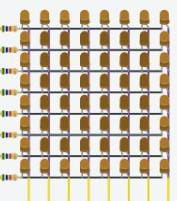
\includegraphics[width=4cm]{manual.jpeg}
\end{document}

